\documentclass[aps,reprint,superscriptaddress,longbibliography,floatfix]{revtex4-2}

\usepackage{amsmath,amssymb}
\usepackage{array}
\usepackage{booktabs}
\usepackage{graphicx}
\usepackage{microtype}
\usepackage{tabularx}
\usepackage{xcolor}
\usepackage[hidelinks]{hyperref}

% Verified manuscript values generated from checked-in machine-readable results.
% Sources:
%   paper/synthetic/results/pevl_results.json
%   paper/data/seed_namespace_audit.json
%   paper/data/ablation/summary.json
%   paper/data/statistical_summary.json
%   paper/data/representation_audit.json
%   paper/data/pevl/trace_preflight_summary.json
%   paper/data/pevl/timed_search_stress_summary.json (when complete)
%   paper/data/pevl/factorial_summary.json (when complete)
%   paper/data/pevl/summary.json (combined admission state)
%
% Prospective preflight, timed-search, and factorial result macros are
% intentionally absent.
% The manuscript exposes those branches only when a results generator validates
% the corresponding analyzer output above and defines:
%   \PEVLPreflightReady
%   \PEVLTimedStressReady
%   \PEVLTimedStressAbstractSentence
%   \PEVLTimedStressResultsParagraph
%   \PEVLTimedStressTableRows
%   \PEVLFactorialReady
%   \PEVLFactorialAbstractSentence
%   \PEVLFactorialResultsParagraph
%   \PEVLFactorialResultsTable
% A terminal suppression uses the same complete family (with an empty table)
% and additionally exposes:
%   \PEVLFactorialSuppressedReady
% A readiness macro must be emitted only with its complete macro family; missing
% members then fail compilation. These macros must never be populated manually
% or with fallback values.

\newcommand{\PEVLSyntheticModes}{5}
\newcommand{\PEVLDrawShiftSharedEvents}{5}
\newcommand{\PEVLDrawShiftMisalignedEvents}{4}

\newcommand{\PEVLHistoricalUnits}{2,800}
\newcommand{\PEVLHistoricalGames}{5,600}
\newcommand{\PEVLHistoricalNarrowedSeeds}{2,800}
\newcommand{\PEVLHistoricalUniqueEngineSeeds}{2,800}
\newcommand{\PEVLHistoricalSeedCollisions}{0}
\newcommand{\PEVLHistoricalOutcomeMismatch}{210}
\newcommand{\PEVLHistoricalOutcomeMismatchPct}{7.50}
\newcommand{\PEVLHistoricalSerializedMismatch}{458}
\newcommand{\PEVLHistoricalSerializedMismatchPct}{16.36}
\newcommand{\PEVLStarmieUnits}{400}
\newcommand{\PEVLStarmieOutcomeMismatch}{191}
\newcommand{\PEVLStarmieOutcomeMismatchPct}{47.75}
\newcommand{\PEVLStarmieSerializedMismatch}{377}
\newcommand{\PEVLStarmieSerializedMismatchPct}{94.25}
\newcommand{\PEVLDipplinUnits}{400}
\newcommand{\PEVLDipplinOutcomeMismatch}{19}
\newcommand{\PEVLDipplinOutcomeMismatchPct}{4.75}
\newcommand{\PEVLDipplinSerializedMismatch}{81}
\newcommand{\PEVLDipplinSerializedMismatchPct}{20.25}
\newcommand{\PEVLOtherHistoricalUnits}{2,000}
\newcommand{\PEVLOtherOutcomeMismatch}{0}
\newcommand{\PEVLOtherSerializedMismatch}{0}
\newcommand{\PEVLHistoricalEffectPP}{2.786}
\newcommand{\PEVLHistoricalCILowPP}{0.679}
\newcommand{\PEVLHistoricalCIHighPP}{4.929}

\newcommand{\PEVLRepresentationOptions}{37,199}
\newcommand{\PEVLRepresentationMultiIdentityStates}{9,776}
\newcommand{\PEVLRepresentationExactCollisions}{0}

\InputIfFileExists{pevl_results_macros.tex}{}{%
  \PackageError{PEVL}{Terminal PEVL result macros are missing}{%
    Run analyze_pevl.py and build_pevl_result_macros.py before compiling.}%
}
\ifdefined\PEVLPreflightReady\else
  \PackageError{PEVL}{Trace-preflight results are not terminal}{%
    A complete terminal preflight analysis is required.}%
\fi
\ifdefined\PEVLTimedStressReady\else
  \PackageError{PEVL}{Timed-search stress results are not terminal}{%
    A complete terminal stress analysis is required.}%
\fi
\ifdefined\PEVLFactorialReady\else
  \PackageError{PEVL}{Factorial admission result is not terminal}{%
    A complete admitted or suppressed factorial branch is required.}%
\fi


\newcommand{\PEVL}{\textsc{pevl}}
\newcommand{\COne}{\textsc{c1}}
\newcommand{\CTwo}{\textsc{c2}}
\newcommand{\CThree}{\textsc{c3}}
\newcommand{\CFour}{\textsc{c4}}
\newcommand{\pp}{percentage points}

\begin{document}

\title{A Validity Ladder for Seed-Matched Evaluation of Game-Playing Agents}

\author{[Author name requires human confirmation]}
\email{[Corresponding-author email required]}
\affiliation{[Affiliation and postal address require human confirmation]}
\date{August 24, 2026}

\begin{abstract}
Paired seeds can increase the precision of stochastic policy comparisons when
the induced seed-level covariance is favorable, but
matching a seed schedule, reproducing an execution, and aligning the same
exogenous events are different requirements.  We introduce the Paired
Evaluation Validity Ladder (\PEVL), an eight-level, fail-closed workflow that
links artifact identity, seed-namespace integrity, schedule parity,
within-arm reproducibility, stochastic-source evidence, event alignment, and a
prespecified statistical admission rule.  A self-contained synthetic testbed
exercises five modes as conformance demonstrations of selected
non-implications.  Seed conversion is first caught at Level 2; injected
wall-clock search and process-global state produce record and context failures
at Levels 4--5 and estimand-relevant source findings at Level 6; and a stateful
draw shift passes within-arm repeat tests but misaligns
\PEVLDrawShiftMisalignedEvents{} of \PEVLDrawShiftSharedEvents{} shared events
at Level 7, after which event-keyed randomness restores alignment.  In a
restricted game-agent case study, a positive but inadmissible historical
one-execution estimate coexisted with
\PEVLHistoricalOutcomeMismatch{}/\PEVLHistoricalUnits{} repeated-control
outcome-record mismatches and
\PEVLHistoricalSerializedMismatch{}/\PEVLHistoricalUnits{} fuller-record
mismatches, confined to two timed-search opponents; the planned mechanistic
decomposition was therefore suppressed.  A prospectively frozen revision then
passed all \PEVLPreflightJobs{} trace-preflight jobs:
\PEVLPreflightTrajectoryUnits{} arm--seed-condition units and
\PEVLPreflightExecutions{} executions across four arms and five opponents had
zero trace, outcome, error, or decision-count mismatches.
\ifdefined\PEVLTimedStressReady\PEVLTimedStressAbstractSentence\space\fi
\ifdefined\PEVLFactorialReady\PEVLFactorialAbstractSentence\space\fi
The contribution is an operational method for deciding which paired claims
black-box evidence permits, not a claim that seed pairing is generally invalid.
\end{abstract}

\maketitle

\section{Introduction: from matched seeds to valid comparisons}

Comparisons between stochastic algorithms are often sharper when the same
random inputs are reused.  If two policies respond similarly to easy and hard
instances, pairing their outcomes by a common random-number construction can
remove between-instance variation from their difference.  Classical results,
however, make the efficiency gain conditional on structural and event-timing
properties rather than on the mere reuse of an integer seed
\cite{glasserman1992crn}.  Streams and substreams provide established tools for
organizing synchronized simulation and independent replications
\cite{lecuyer2002streams}.  A current arXiv preprint likewise shows that paired
seeds can improve precision when seed-level outcomes are favorably correlated
\cite{sharma2025pairedseeds}.  Pairing is therefore valuable when its intended
relationship is implemented and evidenced.

The difficulty is that ``same seed'' can describe several non-equivalent
designs.  Two result files may contain the same scheduled host-language integer
while an engine consumes a narrowed value.  Two byte-identical policies may be
run on the same consumed seed but encounter different wall-clock cutoffs or
process-local state.  Even exact within-policy repetition cannot establish that
two different policies receive the same random quantity for the same semantic
event after one policy takes an extra random draw.  A recent arXiv preprint
formalizes this stateful-draw problem and proposes event-keyed randomness as a
remedy \cite{buffalo2026eventkeyed}.  Schedule matching, repeatable execution,
and cross-policy event alignment must consequently be stated and tested
separately.

This distinction is part of a broader reproducibility problem.  Reproducible
code and methods do not guarantee reproducible findings when essential sources
of variation remain uncontrolled \cite{bouthillier2019reproducible}.  Empirical
reinforcement-learning studies must name their units, sources of variation,
comparison assumptions, and researcher degrees of freedom
\cite{patterson2024empirical}.  Estimation across heterogeneous tasks and
transparent reporting of artifacts and uncertainty are complementary
requirements \cite{agarwal2021statistical,pineau2021reproducibility}.  A
successful rerun of one binary is useful provenance; it is not automatically a
validated paired inference.

The evidentiary gap is especially consequential in black-box game evaluation.
Researchers may have a restricted simulator binary, a seeded entry point,
third-party opponent packages, variable legal-action interfaces, wall-clock
search, and multiprocessing, while lacking authority to replace the engine's
random-number generator.  They can hash artifacts, freeze schedules, repeat
executions, record public traces, and inspect redistributable wrappers, but they
may be unable to expose semantic event identifiers inside the engine.  A
white-box repair such as event-specific streams can then be unavailable even
though a decision about what to report is still required.

We propose the Paired Evaluation Validity Ladder (\PEVL) for that decision.
Its novelty is operational and deliberately narrow: it assembles eight levels
of evidence and applies a prespecified, fail-closed mapping from achieved
evidence to permitted claims.  The ladder does not claim to discover that
common random numbers require assumptions, invent multiple streams, or prove
that a control repeat establishes coupling.  It asks, for a given comparison,
which bytes were run, which seed value was passed at the engine boundary,
whether schedules matched,
whether identical arms reproduced across execution contexts, which stochastic
sources remain, whether shared semantic events were aligned, and what analysis
was authorized if a gate failed.

The paper makes four contributions.  First, it defines the eight-level ladder,
parity-strength vocabulary, and claim-admission rule.  Second, it supplies a
self-contained, standard-library-only synthetic conformance suite in which five
modes demonstrate selected non-implications and an event-keyed construction
repairs a draw-shift failure.  Third, it reanalyzes a restricted game-agent
project in which a positive nominally schedule-matched comparison coexisted with
failed repeated-control parity.  Fourth,
it evaluates a prospectively frozen revision: exact seed conversion, full
public-state/action trace digests, fresh serial repeats, worker-context tests,
a bounded source audit, and a gated fixed-package factorial.  The treatment in
the case study is a missing legal-option-to-observed-item binding; it supplies a
concrete policy difference but is not the title-level contribution.  Throughout,
claims are limited to the tested artifacts, seed schedules, execution settings,
and fixed opponent populations.

Here ``validity'' is deliberately limited to the evidence supporting a
seed-matching and coupling claim.  \PEVL{} does not by itself validate the game
model, the outcome measure, the construction of the policy intervention, or
external generalization; those remain separate scientific questions.

\section{Paired Evaluation Validity Ladder}

The central distinction is
\begin{equation}
 \text{same schedule}\;\nRightarrow\;\text{reproducible executions}
 \;\nRightarrow\;\text{event-aligned coupling}.
 \label{eq:distinction}
\end{equation}
The first relation concerns recorded design variables, the second concerns the
behavior of identical software under repeated execution, and the third concerns
the semantic identity of random events across different policies.  \PEVL
organizes evidence for these questions in the order shown in
Table~\ref{tab:pevl}.  Levels 1--7 are cumulative evidence gates.  Level 8 is a
mandatory decision rule applied to the evidence actually achieved; it cannot
repair a missing lower-level guarantee.

\begin{table*}[t]
\caption{Compressed Paired Evaluation Validity Ladder.  Every pass is scoped to
the tested artifacts, schedules, trajectories, fields, and execution contexts.}
\label{tab:pevl}
\footnotesize
\begin{ruledtabular}
\begin{tabularx}{\textwidth}{c>{\raggedright\arraybackslash}X>{\raggedright\arraybackslash}X>{\raggedright\arraybackslash}X}
Level & Required evidence & Strongest admitted claim & Fail-closed action \\
\hline
1. Artifact identity & Hashes for engine, policies, opponents, protocol, code, and configuration & The evaluated bytes and declared configuration are identifiable & Reject missing or drifting artifacts; do not merge them \\
2. Seed namespace & Scheduled and exact boundary seeds, conversion rule, observable entry-point or stream identity, and collision audit & The claimed engine-boundary seed was supplied and scheduled units remain distinct & Correct the adapter or schedule and rerun \\
3. Schedule parity & Pairwise equality of opponent, order, seat, boundary seed, environment, limits, and schedule fingerprint & A complete matched comparison was attempted & Reject incomplete or unequal pairs without outcome-driven repair \\
4. Identical-arm parity & A/A equality of outcome, errors, decisions, actions, public states, and complete trace digest & Repeatability of the fields compared on tested trajectories & Suppress the affected paired mechanistic contrast \\
5. Repeat/worker parity & Fresh repeats and prespecified worker counts, enqueue orders, pool lifecycles, and all relevant arms & Within-arm reproducibility across tested execution contexts & Freeze a validated context or model execution variation \\
6. Stochastic-source audit & Inventory of RNGs, clocks, concurrency, process/global/native state, numerics, and external state & A bounded account of plausible divergence mechanisms and residual risk & Classify sources as controlled, residual, or estimand changing; downgrade or redesign accordingly \\
7. Cross-arm event alignment & Stable event identifiers and equal values for shared exogenous events after policy branching & Event-aligned CRN language for the covered event set, conditional on its event ontology and random-source marginals & Retain at most bounded seed-matched wording \\
8. Statistical admission & Frozen mapping from achieved levels to estimand, unit, uncertainty, population, and wording & Only the prespecified claim class supported by prior gates & Suppress or downgrade automatically; significance cannot override a failure \\
\end{tabularx}
\end{ruledtabular}
\end{table*}

\begin{figure*}[t]
  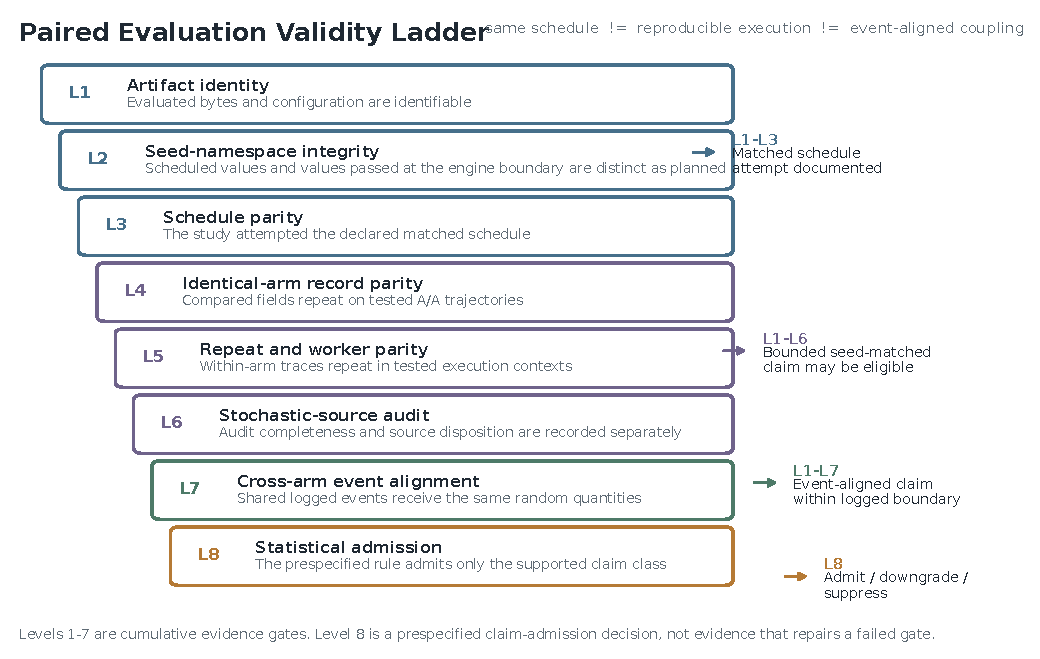
\includegraphics[width=\textwidth]{figures/fig_pevl_01_ladder.pdf}
  \caption{The Paired Evaluation Validity Ladder.  Levels 1--7 accumulate
  scoped evidence about identity, scheduling, reproducibility, stochastic
  sources, and event alignment.  Level 8 applies the frozen admission rule;
  it cannot repair a failed or unavailable gate.}
  \label{fig:pevl-ladder}
\end{figure*}

\subsection{Levels 1--3: identity, namespace, and schedule}

Level 1 binds an observation to artifacts.  Cryptographic hashes cover the
engine, control, candidate, opponent, policy package, protocol, and analysis
code; the record also identifies environment variables, decision limits,
worker settings, and the process start method.  A hash pass establishes which
bytes were evaluated, not what those bytes do.  Missing identity or a byte
mismatch quarantines the affected run.

Level 2 records both the scheduled seed and the exact value passed at the
observable engine boundary.  A host integer may be truncated, reduced modulo a word size,
or mapped into another generator namespace.  The full schedule must therefore
be converted before execution and checked for unintended collisions.  Repeated
use of one scheduled seed within its planned pair is intentional; two distinct
experimental units becoming the same engine seed is not.  The generator or
stream identifier is also part of this level when observable because equal
integers supplied to different generators need not name equal random sequences.
For a black-box entry point, the hashed binary and named entry point identify the
observable interface; whether the engine further transforms or ignores the value
remains blocked internal evidence and must not be described as observed
consumption.

Level 3 checks row-level schedule parity.  Opponent, actual order, physical
seat, exact engine seed, relevant initial-state controls, environment, search
configuration, decision cap, and other prespecified factors must agree between
paired arms.  Expected cells must be complete and fingerprinted.  Passing this
level permits ``schedule matched'' language.  It does not show that either arm
is repeatable or that corresponding random events stay aligned.

\subsection{Levels 4--6: execution reproducibility and source evidence}

Level 4 executes two separately launched byte-identical arms---an A/A
comparison---and compares a hierarchy of records.  An
outcome match is weakest because different action sequences can reach the same
winner.  Error records and decision counts are stronger; action sequences,
public-state sequences, and a complete public-state/action digest are stronger
still.  Reports must name the highest compared field rather than collapse all
forms of agreement into ``deterministic.''  A pass is local to the exercised
trajectories and settings, whereas a single required mismatch falsifies exact
parity on that schedule.

Level 5 varies execution context prospectively.  It includes fresh-process
serial repeats, relevant serial-versus-parallel profiles, worker counts,
enqueue orders, pool lifecycles, and all treatment arms on a frozen subset.
These tests are diagnostics of reproducibility, not randomized experiments on
hardware.  A pass does not generalize to every processor, load, interpreter, or
unvisited state.  A failure requires either a newly frozen context that passes
the intended scope or an analysis in which run-level variation is explicitly
sampled and modeled.

Level 6 audits explicit stochastic sources: engine and library generators,
Python and numerical-library randomness, wall-clock termination, threads and
processes, module globals, native pointers, hardware-sensitive numerics, and
external services.  Static inspection can identify a deadline or a global
agent object but cannot prove that the branch executed or that the named source
was uniquely causal.  Conversely, a clean lexical scan is not proof of
determinism.  Level 6 therefore records two distinct judgments: whether the
audit is complete for its declared boundary, and whether each identified source
is controlled, remains a residual risk, or changes the estimand.  Finding a
source is not itself failure of the audit.  Source evidence determines what
interventions and qualifications are needed; it complements the dynamic trace
gates and should inform which Level-5 contexts are tested.

\subsection{Levels 7--8: event alignment and claim admission}

Level 7 asks the cross-arm question.  When policies branch, every shared
modeled exogenous event must retain a stable identifier and receive the same
random quantity.  Event-keyed counter-based randomness, logged event/value
pairs, or carefully synchronized event-specific streams can provide such
evidence.  Multiple streams and substreams are a white-box strategy, not an
automatic proof that the stream assignment matches semantic events
\cite{lecuyer2002streams}.  Stateful generator guarantees remain bounded by
structure and event timing \cite{glasserman1992crn}; event-keyed constructions
directly target the draw-shift problem \cite{buffalo2026eventkeyed}.  Identical-
arm parity cannot establish this level because two identical arms follow the
same branch and consume the same sequence by construction.
Equal logged values are necessary but not sufficient for a valid stochastic
model: Level 7 remains conditional on the correctness of the event ontology,
the random source's marginal distributions and dependence structure, and any
unlogged event classes.  It validates alignment only within that declared
boundary.

Level 8 freezes the consequence before outcomes are inspected.  It maps the
achieved evidence to an estimand, unit of analysis, interval or test, target
population, and exact wording.  Levels 1--3 alone support provenance and an
attempted schedule-matched description.  Levels 1--6, together with an
appropriate Level-8 rule, can support a bounded seed-matched comparison when
identified execution sources are controlled or explicitly represented in the
estimand.  Levels 1--7 plus Level 8 can support
event-aligned CRN language only for the validated event classes.  A required
Level-4 or Level-5 failure suppresses the affected paired mechanistic contrast;
it cannot be repaired by a small $p$ value, deleting discordant opponents, or
selecting rows after inspection.  \PEVL therefore audits the admissibility of a
pairing claim rather than rejecting pairing.  It does not establish that
seed-level covariance is favorable or that pairing improved precision; those
are separate empirical diagnostics.  When covariance is favorable, the
potential precision gain remains useful, but its claim class must match the
evidence \cite{sharma2025pairedseeds}.

Three qualifications apply throughout.  First, ``pass'' always includes its
scope: bytes, fields, trajectories, seeds, opponents, and execution profiles.
Second, parity must be named at its strongest measured resolution.  Third,
Level 8 governs reporting rather than retroactively making a design valid.  The
ladder is thus an evidence-and-admission system, not a scalar quality score.

Operationally, a \PEVL{} study needs a record that connects these levels rather
than eight independent checklists.  A row or cryptographically linked manifest
should carry the protocol identifier, run identifier, schedule and run
fingerprints, hashes, scheduled and engine-boundary seeds, conversion rule, opponent,
order, seat, environment, decision cap, worker profile, enqueue position,
outcome, errors, decision count, elapsed time, and trace digest.  When Level 7
is possible, the same record must also link semantic event keys to random
values.  This connection matters because a provenance table prepared after an
experiment cannot reconstruct a missing boundary seed, and an aggregate parity
count cannot localize a mismatch whose trace was never retained.  The manifest
is part of the measurement design.

The levels also distinguish a failed gate from a blocked gate.  Failure means
the required comparison was performed and contradicted the equality claim.
Blocked means a prerequisite failed or the needed interface was unavailable,
so the stronger claim was not tested.  For example, a trace mismatch blocks an
event-alignment interpretation even when event logs exist only for a prefix;
an engine without event identifiers leaves Level 7 unavailable even after exact
trace repetition.  Both states constrain reporting, but only the former is
evidence of an observed discrepancy.

Gate evidence uses three statuses: pass, fail, and blocked.  Scoped
qualifications accompany a pass rather than creating additional statuses.
Level 6 separately reports audit completeness and source disposition as
controlled, residual, or estimand changing.  Level 8 then records the reporting
action---admit, downgrade, or suppress.  This vocabulary separates evidence
collection from the consequence imposed on a claim.

\section{Methods}

\subsection{Synthetic conformance and non-implication suite}

We implemented a standard-library-only simulator with deterministic fixtures
for five modes: clean deterministic execution, a stateful draw shift,
wall-clock-bounded search, process-global state, and unsigned-32-bit seed
conversion.  Every mode emits the same eight-level schema, including artifact
identities, scheduled and engine-boundary seeds, schedule fingerprints, compared
fields, execution profiles, source-audit evidence, event/value logs where
available, and the Level-8 decision.  The checked-in JSON and CSV are generated
twice and compared byte for byte.  Clock profiles and worker reuse are injected
as fixed fixture inputs, so the published output is reproducible and does not
depend on the reviewing machine's live scheduler.

The clean mode uses event-keyed SHA-256 values indexed by the engine seed and a
semantic event key.  It is expected to satisfy Levels 1--7 and admit at Level 8
an event-aligned demonstration within its explicitly logged event set.  This
deterministic fixture tests keying and equality, not the marginal quality of
SHA-256 as a production simulator RNG or the correctness of its toy event
ontology.  The
stateful draw-shift mode gives the treatment one additional generator draw
before later events.  Each arm remains exactly reproducible by itself, but
shared event keys can receive different later values.  A second run replaces
the mutable sequence position with the semantic event key; this is the
prespecified white-box remediation motivated by event-keyed randomness
\cite{buffalo2026eventkeyed}.

The wall-clock mode injects different monotonic-clock profiles into byte-
identical arms, causing a bounded search to visit different nodes.  The process-
state mode injects a counter retained by a reused worker while fresh processes
start from the same state.  The seed-conversion mode schedules two distinct
integers that become equal after unsigned-32-bit narrowing.  These fixtures are
counterexamples for selected implications in the audit, not evidence that an
external simulator contains the same defects or a validation of all eight
levels.  We record the first level that catches each constructed failure
and whether the corresponding paired claim is admitted, downgraded, or
suppressed.

The fixtures include negative controls for selected adjacent levels.  The seed-collision
mode keeps within-pair schedules and traces equal so Level 2, rather than an
incidental trace difference, identifies the defect.  The draw-shift mode repeats
each arm under every scripted profile so its Level-7 failure cannot be explained
by within-arm instability.  Clock and process fixtures use byte-identical A/A
artifacts so their Level-4 failures cannot be attributed to a treatment.  The
suite also checks that failure propagation is fail closed: once an exact parity
requirement fails, Level 8 suppresses the affected contrast instead of
manufacturing an effect estimate.  Evidence objects receive deterministic
SHA-256 digests, and the manifest covers the implementation, schema, JSON, and
CSV outputs.

\subsection{Restricted-engine case study and treatment}

The case study uses a two-player, partially observable stochastic card-game
simulator supplied for a competition.  At decision $t$, an agent observes
$o_t$ and a variable collection of legal options
$A_t=\{a_{t1},\ldots,a_{tK_t}\}$.  A neural policy assigns
\begin{equation}
 s_\theta(o_t,a_{tj})=
 h_\theta\!\left(g_\theta(o_t),\phi_\theta(o_t,a_{tj})\right),
 \label{eq:policy-score}
\end{equation}
subject to runtime legality and safety rules.  Imperfect-information systems
such as DeepStack and Pluribus illustrate the broader game-AI setting but are
not empirical comparators here \cite{moravcik2017deepstack,brown2019pluribus}.

The treatment repairs a relational feature.  An ordinary PLAY option stored an
index into the observed hand, while the historical local option vector left the
selected source-card type/ID coordinate at zero.  Pooled hand-identity tokens
and the option's numerical index remained available, but their binding did not.
Permutation-aware set representations provide context for variable-size inputs
\cite{zaheer2017deepsets}; pooling identities does not itself bind an option to
the item it selects.  Invalid-action masking enforces legality but does not
supply missing semantic option features \cite{huang2022invalidmasking}.
Explicit pointers show how a choice can be tied to an input element
\cite{vinyals2015pointer}, and structured action representations can exploit
relations within large finite action sets \cite{chandak2019actionrepresentations}.

The repair resolves an in-range option index to the corresponding observed hand
entry and serializes that entry's public type/ID.  It reveals neither hidden
information nor a unique physical-card serial.  In the retained corpus,
\PEVLRepresentationOptions{}/\PEVLRepresentationOptions{} ordinary PLAY
options lacked the source coordinate under the blind encoder, and
\PEVLRepresentationMultiIdentityStates{} decision states exposed at least two
PLAY identities.  An exact signature over the complete local option-head input
found \PEVLRepresentationExactCollisions{} simultaneous cross-identity
full-vector collision groups.  The evidence therefore establishes a missing
option--item relation, not literal aliasing of complete option vectors.

Four frozen packages define a $2\times2$ case-study treatment.  \COne{} uses the
blind encoder and original weights; \CTwo{} uses the identity encoder with
unchanged original weights; \CThree{} uses the blind encoder and trained
output-side modules; and \CFour{} uses the identity encoder and trained
output-side modules.  \CTwo{} is a representation probe, not a deployable
policy claim, because inherited weights were not trained to interpret the new
coordinate.  Training used one seed, winner/top-episode retained rows, a frozen
trunk, four output-side modules, and a KL anchor to the baseline weights under
the cell's encoder.  Historical batch rounding yielded zero rehearsal rows.
These design facts prevent a general safe-improvement or population-level
learning claim.

\subsection{Retrospective PEVL audit}

The historical experiment preceded \PEVL and is treated as a retrospective
case, not a prospective validation of the ladder.  Its admission rule was frozen
for this reanalysis after the original outcomes already existed, so the case
illustrates fail-closed application rather than prospective prespecification.
At Level 1, raw result files
retain engine and package hashes, although two archived metadata statements
conflict with authoritative member bytes and are disclosed in Appendix B.  At
Level 2, the stored field named \texttt{seed} contains the requested Python
integer.  The adapter actually passed
\texttt{ctypes.c\_uint32(seed).value}; we reconstructed both quantities for all
rows and checked the complete engine-boundary namespace.  The hashed entry point
identifies that observable interface, but the restricted engine does not expose
its internal generator or any further seed transformation.  Level-2 evidence is
therefore bounded at the engine boundary.  At Level 3, candidate and concurrent
control schedules match on the historically recorded opponent, actual order,
physical seat, and requested seed.  Environment, limit, and complete schedule-
fingerprint evidence required by the prospective rule was not retained at the
same resolution, so Level 3 supports recorded-field agreement rather than a full
prospective pass.

The historical four-cell plan ran \CTwo{}, \CThree{}, and \CFour{} in separate
candidate-versus-\COne{} files.  Its admission rule required the repeated
\COne{} outcome, draw, error, and decision-count record to agree across all
three files on every common unit.  Traces had not been captured.  We compared
the three available controls first by terminal record and then by a fuller
serialized tuple.  Level 4 fails if any unit differs; no agreeing subset may be
selected after inspection.

For Level 6, we combined evaluator inspection with a bounded AST source audit
of the exact hashed policy and opponent trees.  The audit searches for explicit
randomness, clocks or deadline identifiers, multiprocessing/threading APIs,
module-global state, and native pointer/state patterns.  Restricted package
source is summarized only by aggregate hit counts and location fingerprints.
A zero-hit category is explicitly not treated as evidence of determinism.
Wall-clock allocation is algorithmically meaningful for Monte Carlo tree search
\cite{baier2016timemanagement}; that literature does not establish that a clock
was the unique cause of any mismatch here.  The restricted engine exposes a
seeded entry point but no semantic random-event IDs or event-specific streams,
so Level 7 cannot be retroactively assessed.  The frozen historical rule maps a
required parity failure to suppression of all cross-cell mechanistic contrasts.

\subsection{Prospective conformance preflight and gated factorial}

The revised protocol was committed before any trace-preflight, timed-search
stress, or five-opponent factorial result was generated or inspected.  It
freezes both engine binaries, the four treatment packages, seven opponent
packages, environment overrides, exact seed ranges, a 2,000-decision cap,
\texttt{spawn} multiprocessing, record fields, stopping rules, resampling
seeds, and the reporting branches.  Once acquisition began, the protocol
permitted no outcome-informed amendment to the population, seed ranges,
estimands, or reporting branches.  Every row records the scheduled Python
integer, conversion rule, exact unsigned-32-bit value passed at the engine
boundary, artifact hashes,
opponent, actual order, physical seat, worker profile, run identifier, public
trace digest, terminal outcome, errors, decision count, and elapsed wall time.

The trace preflight covers five opponents chosen before execution from the
historical packages with zero available repeated-control mismatch: B0,
d842-runtime, master-v1, replay-refresh, and Alakazam with search disabled by
the frozen environment.  They form a new engineering target population, not a
post hoc confirmation of the earlier seven-opponent estimate and not a
probability sample of competition agents.  For each of \COne--\CFour, each
opponent, both actual orders, and 25 seeds per order, we run three profiles: a
fresh serial pool, a second fresh serial pool, and a fresh eight-worker pool.
The preflight therefore contains 1,000 arm--seed-condition units, each observed
under three profiles, and 3,000 execution trajectories.  A mismatch in the
complete public-state/action digest, terminal
result, errors, or decision count suppresses factorial acquisition.

Actual-first seeds use the frozen base plus index $i$; actual-second seeds add
1,000,000 before the same index.  Physical seat is $i\bmod2$ and is held equal
across arms sharing a unit.  Before task dispatch, the evaluator converts every
scheduled value with \texttt{seed \& 0xffffffff}, asserts uniqueness across
distinct seed-condition units after conversion while permitting planned reuse
within an arm comparison, and fingerprints the ordered task list.  The
public digest is computed from canonical serialized public observations and
chosen actions at every decision.  Full restricted traces are retained locally
for possible first-divergence inspection, whereas only their safe digests and
summary fields enter the review package.

The timed-search diagnostic is separate from the factorial population.  It
runs \COne{} against Starmie and Dipplin for both orders and 50 seeds per order.
Each of the 200 opponent--order--seed clusters is executed in a fresh one-worker
pool with forward enqueue, one worker with reverse enqueue, four workers with
forward enqueue, and four workers with reverse enqueue, for 800 executions.
The primary endpoint is agreement of all four complete trace digests.  Secondary
endpoints are first-divergence position and actor, decision-count disagreement,
terminal-outcome disagreement, errors, and elapsed-time summaries.  Worker and
enqueue comparisons are descriptive diagnostics, not randomized hardware
effects.

Only a complete preflight pass authorizes the factorial.  The preflight and
factorial use disjoint frozen seed ranges; preflight observations are gate
diagnostics and are not part of the factorial estimands.  Each of \CTwo{},
\CThree{}, and \CFour{} is compared with a separately executed \COne{} over the
five-opponent population, two orders, and 200 paired units per stratum.  The
three candidate--control comparisons share 2,000 common seed-condition units
and contain 12,000 games in total.  Any error, cap exception, incomplete
schedule, hash or sentinel drift,
seed collision, schedule mismatch, or one repeated-\COne{} record mismatch
suppresses every factorial contrast.  Runs are not stopped for effect size, and
no opponent, seed, or row may be removed after result inspection.

\subsection{Estimands and statistical admission}

For the timed-search diagnostic, the seed-condition containing four executions
is the resampling cluster.  To describe how the observed fixed-schedule rate
changes under empirical reweighting of those clusters, we use 100,000 resamples
of whole clusters with frozen seed 2026083118.  Cluster resampling preserves
within-cluster dependence \cite{field2007clustered}; here it defines an
empirical stability interval, not a confidence interval for an unsampled seed or
opponent population.  A single mismatch falsifies exact reproducibility on the
exercised schedule, while the observed rate describes its frequency in that
finite test.

For an admitted factorial, let $\bar W_{ak}$ be the mean binary win indicator
for arm $a$ in opponent-by-order stratum $k$, with losses and draws coded zero.
The ten strata receive equal weight.  The primary total intervention is
\begin{equation}
 \widehat\Delta_{\mathrm{total}}=
 \frac{1}{10}\sum_{k=1}^{10}
 (\bar W_{\mathrm{C4},k}-\bar W_{\mathrm{C1},k}).
\end{equation}
Secondary fixed-package contrasts are the representation contrast
$\tfrac12[(\mathrm{C2}-\mathrm{C1})+(\mathrm{C4}-\mathrm{C3})]$, the training contrast
$\tfrac12[(\mathrm{C3}-\mathrm{C1})+(\mathrm{C4}-\mathrm{C2})]$, and the package
interaction $\mathrm{C4}-\mathrm{C3}-\mathrm{C2}+\mathrm{C1}$, with each symbolic
difference understood as the same equal-stratum mean.  The repeated-control gate
requires the three separately executed \COne{} records to agree, after which
they define the common fixed-package \COne{} term.  The labels do not denote
population-level representation or training effects: only one trained package
per encoder and one training seed were used.  Empirical stability intervals use
100,000 paired within-stratum resamples with seed 2026083117.  The exact
two-sided McNemar calculation is a secondary fixed-schedule discordance
diagnostic, not a population-inference claim.  This estimation-first design
names the observed variation and comparison assumptions without treating
significance as a validity test
\cite{patterson2024empirical,agarwal2021statistical}.

The Level-8 branch is selected before effect inspection.  Preflight failure
means no factorial acquisition.  Acquisition or repeated-control failure means
all effects are suppressed.  A full pass permits the prespecified estimates
only for the exact five opponents, frozen seed schedule, packages, and execution
configuration.  The stability intervals describe empirical sensitivity to
reweighting those observed seed-condition units; they do not extend the target
to an unsampled population.
Even then the restricted engine remains below Level 7, so permitted language is
``seed matched,'' never an event-aligned counterfactual.

\section{Results}

\subsection{Synthetic failure-mode detection}

The synthetic suite produced its checked-in matrix deterministically.  Clean
execution passed all eight levels: artifacts and seeds were identified, the
schedule matched, identical arms and worker profiles reproduced full traces,
the event-keyed source was explicit, and all covered shared event keys received
equal values.  The fixture therefore admitted an event-aligned demonstration
within its small logged event set.

The unsigned-32-bit fixture failed first at Level 2.  Two distinct requested
seeds narrowed to one engine value, even though each within-seed pair had equal
schedules, identical-arm repetition, and aligned events.  This is the intended
counterexample to using A/A repetition as a namespace audit: exact repetition
cannot reveal that two nominal experimental units are duplicates at the engine
boundary.  Level 8 rejected the collided schedule before statistical analysis.

Injected wall-clock search and process-global state failed at Level 4.  In the
clock fixture, byte-identical arms generated different public-state/action
records under different fixed clock profiles; repeat/worker comparison and the
source audit also identified the bounded timing mechanism at Levels 5 and 6.
In the process fixture, fresh-process repeats agreed but reused-worker execution
inherited a counter and diverged.  Its source audit exposed the controlled
module-global state.  Both affected comparisons were suppressed.  Because the
fixtures inject these mechanisms, the attribution is exact inside the testbed;
it does not license the same attribution for the restricted engine.

The stateful draw-shift mode supplied the complementary boundary.  Artifact,
namespace, schedule, identical-arm trace, repeat/worker, and source-audit gates
all passed.  Nevertheless, one treatment-only draw changed
\PEVLDrawShiftMisalignedEvents{} of the
\PEVLDrawShiftSharedEvents{} later shared semantic event values.  Level 7 alone
caught the failure.  Replacing mutable sequence position with
\texttt{SHA256(seed, semantic-event-key)} restored equality for all shared
event keys.  The result shows why no lower-level gate is sufficient by itself:
Level 2 catches a collision that trace repetition misses, Levels 4--6 catch
execution-context failures, and Level 7 catches cross-arm event drift that
perfect within-arm reproduction misses.

\begin{figure*}[t]
  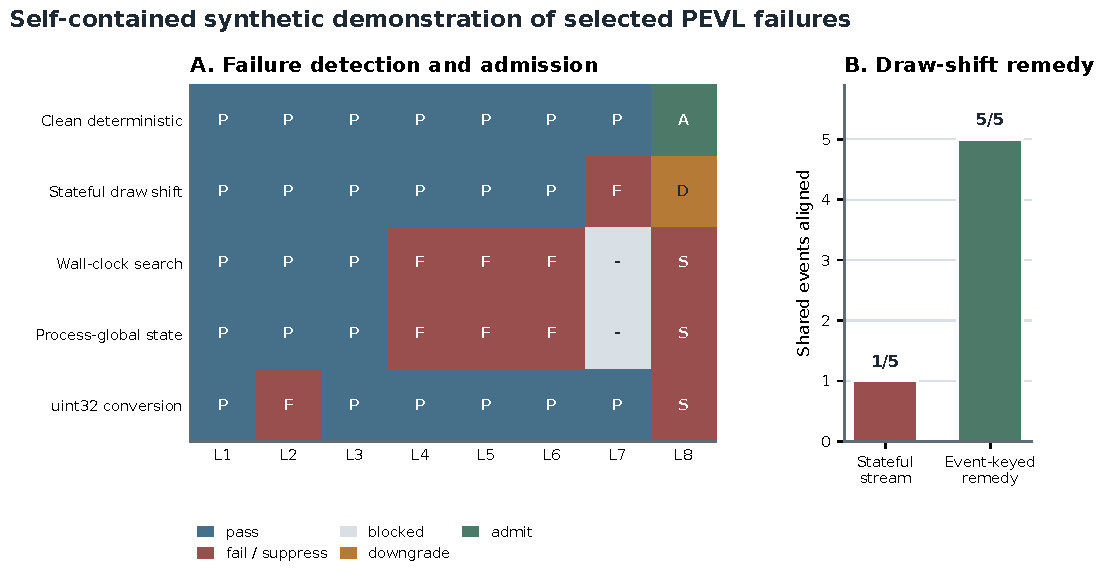
\includegraphics[width=\textwidth]{figures/fig_pevl_02_synthetic.pdf}
  \caption{Synthetic validation of the ladder.  Panel A records the
  prespecified level status for each controlled failure mode.  Panel B shows
  that replacing a stateful stream with event-keyed randomness restores
  equality for the logged shared events after a treatment-only draw shift.}
  \label{fig:pevl-synthetic}
\end{figure*}

\subsection{Retrospective restricted-engine audit}

The artifact inventory was sufficient to identify the historical engine and
packages, subject to the disclosed stale metadata.  Seed reconstruction changed
\PEVLHistoricalNarrowedSeeds{}/\PEVLHistoricalUnits{} requested values under
unsigned-32-bit narrowing.  The resulting namespace contained
\PEVLHistoricalUniqueEngineSeeds{} unique consumed values and
\PEVLHistoricalSeedCollisions{} collision groups.  Thus the historical defect
was inaccurate field semantics and failure to store the exact consumed value,
not a collision within those 2,800 units.  Candidate and control schedules
matched the recorded opponent, actual order, physical seat, and requested seed.

Before the repeated-control audit, the historical \CFour--\COne{} file yielded
an equal-stratum one-execution win-rate difference of
+\PEVLHistoricalEffectPP{} \pp{} with a conditional resampling interval
[+\PEVLHistoricalCILowPP{}, +\PEVLHistoricalCIHighPP{}].  That attractive
number is retained only to show the consequence of the gate.  Its interval
conditions on one realized execution and omits run-to-run search variation; it
is neither the paper's primary result nor a decomposition of representation and
training.

The Level-4 audit failed.  At least one of the three repeated \COne{} controls
disagreed on the terminal outcome/draw/error record in
\PEVLHistoricalOutcomeMismatch{}/\PEVLHistoricalUnits{} units
(\PEVLHistoricalOutcomeMismatchPct\%) and on the fuller serialized record in
\PEVLHistoricalSerializedMismatch{}/\PEVLHistoricalUnits{} units
(\PEVLHistoricalSerializedMismatchPct\%).  Historical traces were absent, so
neither action parity nor public-state/action digest parity can be reconstructed.
The mismatch was confined to the two timed-search opponent packages.

Starmie contributed \PEVLStarmieOutcomeMismatch{}/\PEVLStarmieUnits{}
outcome-record mismatches (\PEVLStarmieOutcomeMismatchPct\%) and
\PEVLStarmieSerializedMismatch{}/\PEVLStarmieUnits{} serialized-record
mismatches (\PEVLStarmieSerializedMismatchPct\%).  Dipplin contributed
\PEVLDipplinOutcomeMismatch{}/\PEVLDipplinUnits{}
(\PEVLDipplinOutcomeMismatchPct\%) and
\PEVLDipplinSerializedMismatch{}/\PEVLDipplinUnits{}
(\PEVLDipplinSerializedMismatchPct\%), respectively.  Each of B0,
d842-runtime, master-v1, replay-refresh, and Alakazam-no-search had zero
available mismatches across 400 units.  Those zero historical summaries
motivated a newly frozen population; they do not retroactively rescue the
seven-opponent analysis.

\begin{table*}[t]
\caption{Retrospective \PEVL{} audit.  Panel B reports available record parity;
complete public traces were not captured historically.}
\label{tab:retrospective}
\footnotesize
\begin{ruledtabular}
\begin{tabularx}{\textwidth}{l>{\raggedright\arraybackslash}Xl>{\raggedright\arraybackslash}X}
Level or opponent & Observed evidence & Status & Consequence \\
\hline
\multicolumn{4}{l}{\textit{Panel A: level-by-level audit}}\\
1 & Engine and package hashes retained; stale metadata disclosed & bounded pass & Evaluated bytes identifiable \\
2 & 2,800 requested values narrowed; 2,800 unique consumed values; zero collisions & pass & Namespace distinct, historical field label corrected \\
3 & Opponent, order, seat, and requested seed matched within files & pass & Attempted schedule match only \\
4 & 210 outcome-record and 458 serialized-record mismatch units & fail & Cross-cell mechanistic contrasts suppressed \\
5 & No historical fresh-repeat/worker trace design & unavailable & No execution-context reproducibility claim \\
6 & Clock deadlines, process-pool dispatch, and native/process-local state identified & bounded audit & Timing association; no sole-cause claim \\
7 & Engine exposes no semantic event identifiers & unavailable & No event-aligned or counterfactual wording \\
8 & Frozen repeated-control rule applied & suppress & Seven-opponent factorial decomposition rejected \\
\hline
\multicolumn{4}{l}{\textit{Panel B: repeated-control mismatch localization}}\\
B0 & 0/400 outcome; 0/400 serialized & observed parity & Scope limited to available fields \\
d842-runtime & 0/400 outcome; 0/400 serialized & observed parity & Scope limited to available fields \\
master-v1 & 0/400 outcome; 0/400 serialized & observed parity & Scope limited to available fields \\
replay-refresh & 0/400 outcome; 0/400 serialized & observed parity & Scope limited to available fields \\
Alakazam-no-search & 0/400 outcome; 0/400 serialized & observed parity & Scope limited to available fields \\
Starmie & 191/400 outcome; 377/400 serialized & fail & Timed-search diagnostic population \\
Dipplin & 19/400 outcome; 81/400 serialized & fail & Timed-search diagnostic population \\
\end{tabularx}
\end{ruledtabular}
\end{table*}

\begin{figure*}[t]
  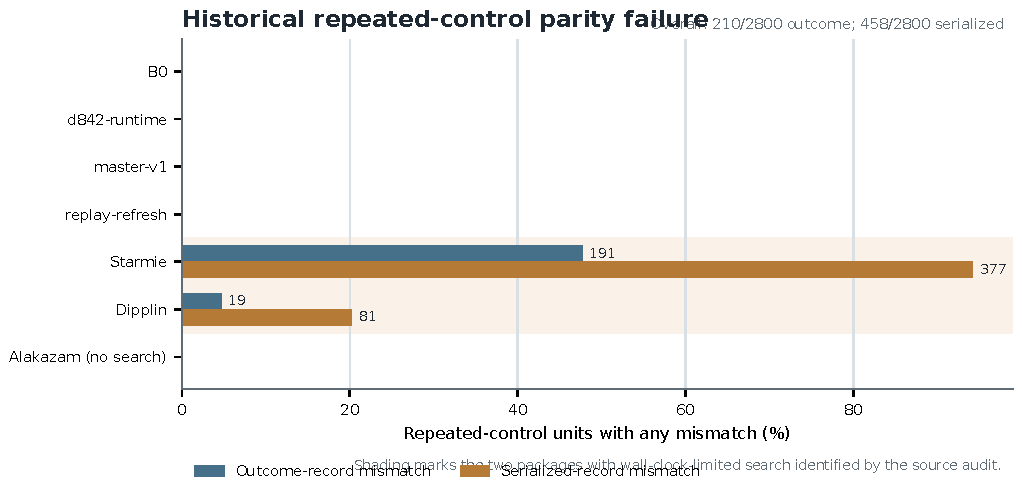
\includegraphics[width=\textwidth]{figures/fig_pevl_03_historical_parity.pdf}
  \caption{Historical repeated-control parity audit by opponent.  Outcome-
  record and fuller serialized-record mismatches were confined to the two
  timed-search packages; complete historical traces were unavailable, so the
  figure does not establish action- or state-sequence parity elsewhere.}
  \label{fig:pevl-historical}
\end{figure*}

The bounded package scan found explicit random interfaces and module/global and
native-state patterns across the inspected trees.  Clock/deadline patterns
appeared in Starmie, Dipplin, and the Alakazam source tree; the last package ran
under \texttt{NO\_SEARCH=1}, so static presence does not establish branch
execution.  No explicit package-local multiprocessing/threading pattern was
found, while separate inspection of the evaluator showed process-pool task
dispatch and the runtime wrapper exposed process-local native state.  The
historical concentration is consistent with timing sensitivity, but scheduler,
native, and hidden engine behavior were not isolated by a controlled
intervention.  Level 6 therefore supports a plausible-mechanism account, not a
unique causal attribution.

The Level-8 consequence is categorical.  The favorable \CFour--\COne{}
observation cannot be attributed to the identity encoder, retraining, or their
interaction.  The planned \CTwo--\COne{}, \CThree--\COne{}, \CFour--\COne{},
\CFour--\CTwo{}, \CFour--\CThree{}, and difference-in-differences contrasts are
suppressed.  A post hoc restriction to the five agreeing historical opponents
is appendix-only, descriptive, and receives no interval or test.

\subsection{Prospective trace preflight}

The prospective seed audit covered every trace, stress, and factorial schedule
before acquisition.  All scheduled values were already within unsigned-32-bit
range, conversion changed none, no unintended collision occurred, and the
prospective consumed namespace did not overlap the historical consumed values.
All 13 frozen artifact bindings---the two engine binaries, four treatment
packages, five preflight opponents, and two timed-search opponents---matched
their expected file or canonical tree digest.

The trace preflight passed in full.  All \PEVLPreflightJobs{} arm--opponent jobs
completed, comprising \PEVLPreflightTrajectoryUnits{} arm--seed-condition
trajectories and \PEVLPreflightExecutions{} executions.  Across the two fresh
serial profiles and the eight-worker profile, there were
\PEVLPreflightTraceMismatches{} complete public-state/action trace mismatches,
\PEVLPreflightOutcomeMismatches{} terminal-record mismatches,
\PEVLPreflightErrorMismatches{} error mismatches, and
\PEVLPreflightDecisionMismatches{} decision-count mismatches.  This result is stronger
than the historical outcome-only evidence because it compares full public
traces, covers every treatment arm, and changes the worker context.

The pass was complete at both natural aggregations.  Each arm contributed 250
seed-condition trajectories and 750 executions, and each of the five opponents
contributed 200 trajectories spanning all four arms and 600 executions.  Thus
the aggregate zero is not the result of an omitted arm or opponent.  Every raw
job retained its source digest, and the summary recorded the expected and
completed job counts as 20 and 20.  The protocol commit and execution commit
were also carried into the summary, separating the frozen design from the code
revision that performed acquisition.

\begin{table*}[t]
\caption{Prospective execution-parity evidence available in the current
machine-generated record.  Each preflight arm covers five opponents, two
orders, 25 seeds per order, and three execution profiles.}
\label{tab:prospective}
\footnotesize
\begin{ruledtabular}
\begin{tabular}{lrrrrrl}
Stage/arm & Seed-condition units & Executions & Trace mismatch & Outcome mismatch & Decision/error mismatch & Admission \\
\hline
Preflight \COne & \PEVLPreflightUnitsPerArm & \PEVLPreflightExecutionsPerArm & 0 & 0 & 0 & pass \\
Preflight \CTwo & \PEVLPreflightUnitsPerArm & \PEVLPreflightExecutionsPerArm & 0 & 0 & 0 & pass \\
Preflight \CThree & \PEVLPreflightUnitsPerArm & \PEVLPreflightExecutionsPerArm & 0 & 0 & 0 & pass \\
Preflight \CFour & \PEVLPreflightUnitsPerArm & \PEVLPreflightExecutionsPerArm & 0 & 0 & 0 & pass \\
\hline
Full preflight & \PEVLPreflightTrajectoryUnits & \PEVLPreflightExecutions & 0 & 0 & 0 & admit acquisition \\
\ifdefined\PEVLTimedStressReady\PEVLTimedStressTableRows\fi
\end{tabular}
\end{ruledtabular}
\end{table*}

The observed pass is scoped to the exact five packages, four arms, 50 seeds per
opponent, three profiles, and recorded trace schema.  It establishes Levels
1--5 for that preflight scope; the accompanying source inventory supplies a
bounded Level-6 audit.  It does not prove behavior on different hardware or
loads, and it cannot establish Level 7 inside the restricted engine.  Under the
frozen Level-8 rule, the pass admits factorial acquisition, not a favorable
effect claim.

\ifdefined\PEVLTimedStressReady
\subsection{Prospective timed-search stress test}
\PEVLTimedStressResultsParagraph
\begin{figure}[t]
  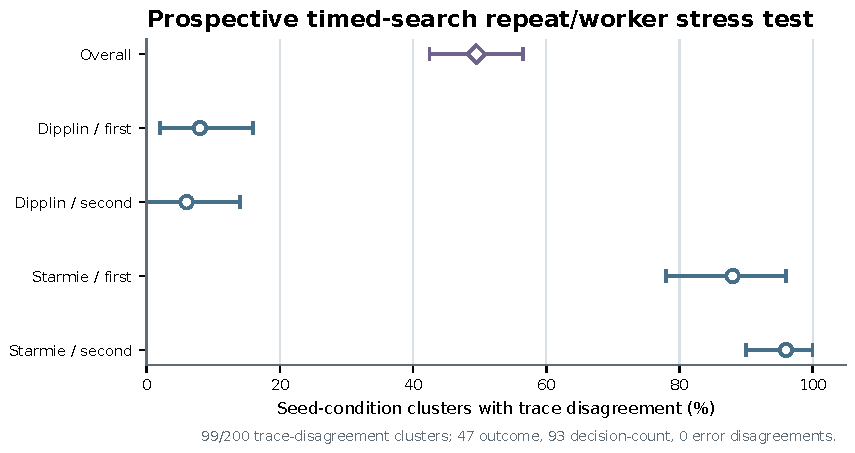
\includegraphics[width=\columnwidth]{figures/fig_pevl_04_stress.pdf}
  \caption{Prospective trace-disagreement rates in the separately frozen
  timed-search diagnostic.  Intervals resample whole seed-condition clusters;
  any observed mismatch rejects exact parity on this stress schedule.}
  \label{fig:pevl-stress}
\end{figure}
\fi

\ifdefined\PEVLFactorialReady
\subsection{Gated factorial result}
\PEVLFactorialResultsParagraph
\PEVLFactorialResultsTable
\ifdefined\PEVLFactorialAdmitted
\begin{figure}[t]
  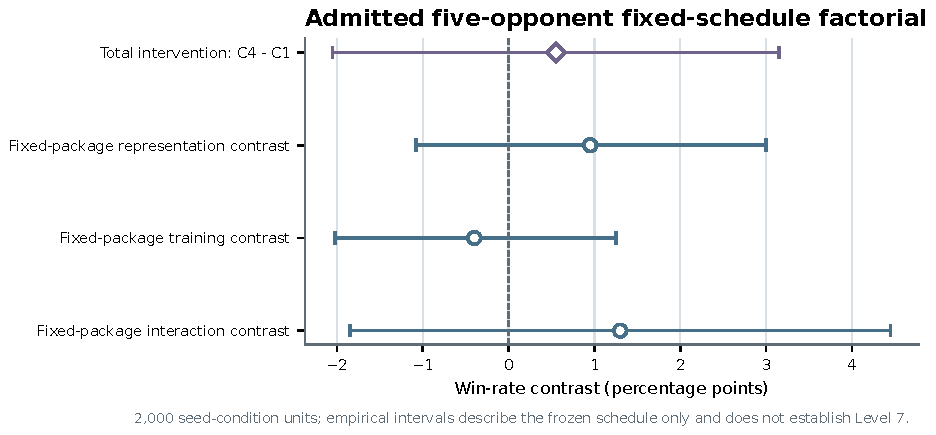
\includegraphics[width=\columnwidth]{figures/fig_pevl_05_factorial.pdf}
  \caption{Prespecified contrasts from the admitted five-opponent factorial.
  Points are equal-stratum win-rate differences and bars are paired bootstrap
  95\% intervals.  Admission remains scoped below event-alignment Level 7.}
  \label{fig:pevl-factorial}
\end{figure}
\fi
\fi

\section{Discussion: what the ladder changes}

\subsection{Pairing is conditional, not rejected}

The results argue against an unconditional vocabulary, not against paired
evaluation.  When seed-level outcomes are positively correlated, pairing can
substantially improve precision, as the current paired-seed preprint emphasizes
\cite{sharma2025pairedseeds}.  \PEVL asks whether the implemented design
supports the correlation and interpretation being used.  A schedule may be
perfectly matched even when an engine adapter collapses nominal units or an
opponent's clock changes the realized path.  Conversely, a package can contain
explicit randomness and still reproduce exactly on a prespecified execution
scope.  Evidence should determine the claim rather than a categorical label
such as ``seeded'' or ``deterministic.''

The synthetic suite makes the conditional structure concrete.  Namespace
integrity and identical-arm parity are logically independent: the conversion
fixture repeats perfectly while duplicating a unit at the engine boundary.
Within-arm reproducibility and cross-arm event alignment are also independent:
the draw-shift fixture repeats perfectly within each policy while four later
shared events change values.  A single omnibus reproducibility check would miss
at least one of these failures.  The ladder's ordering is useful because each
gate has a distinct repair: correct the namespace, change the execution design,
instrument a source, or introduce event-specific randomness.

\subsection{Black-box validation complements white-box remedies}

Where a simulator is modifiable, event-keyed random values or carefully
assigned event-specific streams are stronger than evidence based only on
repetition \cite{buffalo2026eventkeyed,lecuyer2002streams}.  They make the
coupling target part of the model.  Yet many empirical systems include closed
binaries, licensed data, third-party agents, or platform-owned interfaces.  In
those cases researchers cannot always implement the strongest remedy.  The
scientific alternative is not to assume the guarantee; it is to delimit what
the available evidence supports.

\PEVL provides that black-box path.  Hashes and exact engine seeds establish
identity and namespace.  Schedule fingerprints show the attempted match.
Trace-level A/A tests reveal whether public behavior repeats, and execution-
profile tests probe worker sensitivity.  A source inventory identifies clocks,
state, and residual risk without overclaiming.  If event IDs remain hidden, the
result stops at seed-matched, implementation-conditional language.  This is a
weaker claim than event-aligned CRN, but it is auditable and often scientifically
useful.

\subsection{Control parity is one rung, not a certificate}

The historical and prospective case studies show both sides of control parity.
Historically, outcome-level disagreement exposed a fatal problem before an
attractive mechanistic decomposition was reported.  Prospectively, complete
trace agreement across two fresh serial runs and an eight-worker run supplies
substantially stronger evidence for the new five-opponent scope.  Neither result
supports a universal statement.  The historical mismatch does not prove that
all seed matching fails, and the prospective pass does not prove event
alignment after policies branch.

Trace resolution also changes what is learned.  Terminal agreement can conceal
different action sequences, different public states, or errors that happen to
produce the same winner.  A digest mismatch, when linked to a retained trace,
can be localized to the first divergent decision and acting side.  This makes
the gate diagnostic rather than merely punitive.  But a digest is only as
complete as its serialization schema, so the compared public fields and any
excluded restricted state must be documented.

\subsection{Fail-closed reporting is a scientific result}

The historical \CFour--\COne{} observation illustrates why admission must
precede interpretation.  Its conditional interval looked favorable.  After
the separately executed controls disagreed, retaining the decomposition would
have allowed process variation to masquerade as representation or training.
Deleting Starmie and Dipplin after seeing the mismatch would have changed the
target population and rewarded a favorable rescue.  Suppression preserves the
failure as evidence about the evaluation method.

Fail-closed does not mean discarding data.  The mismatch counts, opponent
localization, historical point estimate, and source-supported mechanisms remain
reportable with bounded labels.  What disappears is the unauthorized inference.
This distinction encourages publishing validation failures rather than hiding
them and separates redesign from post hoc repair.  A prospectively redefined
five-opponent population is a new study target, not a reanalysis that confirms
the old one.

\subsection{Interpretation of the representation treatment}

The option--item repair is factually grounded: an observed index can be bound to
the public identity of the item it selects.  The zero exact within-state
full-vector collisions do not make the historical representation relationally
sufficient, because pooled item identities and local indices still omit their
mapping.  At the same time, correcting the coordinate does not imply a gameplay
benefit.  \CTwo{} has not learned how to use it, training used one outcome-
selected corpus and one seed, and runtime logic can mediate neural scores.

This is precisely why the four cells matter.  In principle they separate the
total fixed-package intervention into representation, training, and interaction
terms.  In practice that language is admitted only after the preflight and
repeated-control gates.  The historical gate failure blocks the decomposition;
the prospective preflight pass authorizes acquisition but does not supply the
effect.  The ladder therefore allows the project to describe what was built and
what reproduced without converting engineering uniqueness into a causal claim.

\subsection{Open-science value under restricted access}

The standalone synthetic suite makes every level, failure, and event-keyed repair
independently executable.  The restricted case releases protocols, processed
audit rows, hashes, safe trace diagnostics, analysis code, and the exact claim
rules, subject to final rights approval.  This layered release follows the
broader goals of reproducible artifact reporting
\cite{pineau2021reproducibility}.  Dataset and artifact documentation should
state intended use, composition, provenance, and access constraints rather than
implying that a public aggregate recreates restricted raw material
\cite{gebru2021datasheets}.

The split between standalone and restricted evidence is not ideal, but it is explicit.
An independent reader can reproduce the logical counterexamples, verify
processed counts, inspect protocols, and confirm that manuscript branches are
machine gated.  Replaying the exact game trajectories still requires lawful
access to the engine, opponents, policy packages, and protected game material.
This distinction prevents ``open code'' from being used as shorthand for full
computational reproducibility when essential third-party components remain
closed.

\subsection{Use beyond game-agent evaluation}

Although the terminology here follows policies, opponents, and trajectories,
the ladder applies more broadly to paired stochastic computation.  A simulation
study comparing interventions, a randomized optimizer benchmark, or an agentic
software evaluation can each distinguish an input schedule from repeatable
execution and semantic alignment.  The appropriate trace may be a sequence of
public simulator states, solver callbacks, tool invocations, or modeled random
events.  The appropriate execution profiles may vary thread count, accelerator,
queue order, or service process lifetime.  What transfers is the admission
logic, not the game-specific fields.

This broader use requires adaptation rather than mechanical adoption.  Floating-
point kernels may need tolerance-based records alongside exact hashes; networked
systems may need versions and response identities for external services; long-
running simulations may need checkpoint and restart provenance.  In each case
the equality relation must be specified before comparison.  A tolerance can be
scientifically appropriate, but choosing it after seeing a discrepancy defeats
the gate.  Likewise, a trace that excludes a state component can establish
parity only for the serialized projection.  \PEVL{} is most useful when it
forces these design choices into the protocol instead of leaving them implicit
in analysis code.

\section{Limitations}

First, \PEVL is evaluated in one synthetic suite and one restricted game
domain.  The suite is designed to separate known logical failure modes, not to
estimate their prevalence.  Its clocks and process state are injected fixed
fixtures rather than measurements of a live operating system.  Other domains
may require additional fields, event classes, hardware diagnostics, or levels;
the proposed ladder is not yet a universal standard.

Second, the restricted engine cannot expose semantic event identifiers or
independent event streams.  No restricted-engine result can satisfy Level 7,
even if every observed trace repeat passes.  A passing result remains seed
matched, finite-population, and implementation conditional.  Hidden engine
state and unlogged event classes remain outside the public trace boundary.

Third, both historical and prospective opponent groups are fixed engineering
populations rather than probability samples.  The five preflight/factorial
opponents were frozen after the historical audit as a new target because their
available repeated-control records agreed.  They do not represent the full
competition field, and their prospective behavior cannot confirm the earlier
seven-opponent observation.  Timed-search Starmie and Dipplin are retained as a
separate diagnostic population.

Fourth, historical traces and per-game timing were not captured.  Source and
wrapper inspection supports the relevance of monotonic deadlines, process-pool
dispatch, and native/process-local state, but no controlled historical
intervention isolated wall-clock timing as the unique cause.  The concentration
of mismatches is therefore associated with timed-search packages, not proof of
a sole mechanism.  Static no-hit results likewise do not prove absence.

Fifth, the treatment evidence has its own boundaries.  Training used one seed,
winner/top-episode retained data, a frozen trunk, and no realized rehearsal
rows.  \CTwo{} is an untrained-feature probe.  Original source replay
observations for part of the retained feature corpus are missing, and the
nominal temporal holdout is empty.  These constraints limit statements about
representation learning, offline agreement, and generalization.

Sixth, the tournament engine and source, opponent implementations, card data,
deck material, full restricted traces, private replay observations, and
possibly policy weights cannot be redistributed under the currently established
rights.  Exact end-to-end replication requires separately authorized access.
Hashes and processed summaries support identity and bounded verification, not a
substitute reconstruction of protected artifacts.

Finally, authorship, affiliation, corresponding-author ORCID, CRediT roles,
funding, conflicts, acknowledgments, complete historical AI-tool use, release
ownership, license approval, repository citation, and archival DOI remain human
submission blockers.  They are left explicit rather than inferred from Git
history or project files.

\section{Conclusion}

Matching a seed schedule is not the same as reproducing executions, and neither
establishes event-aligned coupling after policies branch.  \PEVL connects these
distinct questions to eight evidence and admission levels.  The standalone synthetic
suite shows that seed collisions, clock and process state, and stateful draw
shifts require different gates.  The restricted case shows the value of failing
closed: a favorable one-execution estimate did not survive its historical
repeated-control requirement, whereas a newly frozen five-opponent preflight
passed 1,000 full-trace trajectory checks across serial and worker profiles.
For black-box paired studies, we recommend recording exact consumed seeds,
testing identical arms and relevant execution contexts at trace level, auditing
stochastic sources, distinguishing seed matching from semantic event alignment,
and suppressing every contrast whose required gate fails.

\begin{acknowledgments}
Acknowledgment of the competition organizer, engine provider, data contributors,
compute providers, and human reviewers requires permission and author
confirmation.  Funding and grant identifiers have not been established from
repository evidence and must be supplied or explicitly declared absent.

\medskip
\noindent\textit{Artificial-intelligence assistance disclosure.}
OpenAI Codex, operating with a GPT-5-family model whose exact deployed snapshot
identifier was not exposed in the session, provided substantive assistance in
August 2026.  Under human direction it helped audit repository artifacts; draft
and review Python, \LaTeX, and release files; implement statistical checks and
visualizations; verify bibliographic metadata; and draft and edit prose.
Bounded worker agents performed evidence and literature audits.  Every admitted
number was required to trace to retained raw evidence or a frozen prospective
protocol, with checks through hashes, executable regeneration, tests, source
inspection, compilation, and full-page rendering.  No generative-image model
was used for this manuscript.  Human authors remain responsible for all content
and must add any substantive earlier AI use not recoverable from repository
history.  AI systems are not authors.
\end{acknowledgments}

\section*{Author contributions}

CRediT roles for conceptualization, methodology, software, validation, formal
analysis, investigation, data curation, visualization, writing, supervision,
administration, and funding acquisition require author-confirmed names.  They
are intentionally not inferred from Git history.

\section*{Competing interests}

No reliable conflict statement was found in the repository.  Every author must
confirm relevant financial and nonfinancial interests before submission; the
corresponding author may state that none exist only after that review.

\section*{Data Availability Statement}

The component prepared for public release contains the synthetic simulator,
deterministic fixtures, eight-level JSON/CSV outputs, schema, and verification
manifest.  Its redistribution remains subject to the final rights and license
approval described below.  The restricted case-study component is designed to
contain protocols, artifact hashes,
seed-namespace and stochastic-source audits, processed historical parity rows,
safe prospective trace diagnostics, and analysis code.  These materials allow
independent inspection of the ladder and reaggregation of released counts, but
not reconstruction of protected game trajectories.

The tournament engine and source, card database, deck files, private replay
observations, full traces, and third-party opponent packages are not
redistributed because of organizer terms, third-party rights, and privacy
constraints.  Exact gameplay regeneration requires separately authorized
access to the engine and packages identified by hash.  Policy-weight release
also remains subject to rights review.  Repository DOI, archival location,
maintainer contact, license, and any controlled-access procedure must be
supplied before submission.  A formal data/software citation with creators,
title, year, version, repository, and persistent identifier must then be added;
those facts are not inferred here.

\appendix

\section{Formal claim and resampling details}

Let $R_{aikr}$ denote the complete recorded result for arm $a$, stratum $k$,
seed-condition $i$, and execution profile $r$.  Level-4 parity compares two
byte-identical arms at fixed $(k,i,r)$; Level-5 parity compares the same arm and
seed condition across a prespecified set of $r$.  The record is ordered by
strength: terminal outcome, errors, decision count, action sequence, public-
state sequence, and the digest of the full public-state/action sequence.  An
equality statement applies only through the last field actually compared.

For timed-search stress, the bootstrap samples seed-condition identifiers and
retains all four execution profiles within each sampled cluster.  Percentile
limits are computed separately by opponent and actual order.  This preserves
the repeated-execution dependence rather than treating 800 games as independent
\cite{field2007clustered}.  First-divergence positions and actors are descriptive
conditional summaries among mismatched clusters.

For the factorial, one bootstrap replicate samples paired-unit indices with
replacement independently within each of the ten opponent-by-order strata,
recomputes the four arm means, forms each contrast, and averages strata equally.
The interval is the 2.5 and 97.5 percentiles.  Exact McNemar inference for the
primary binary contrast conditions on discordant directions.  No equivalence
claim follows merely because an interval contains zero, and no significance
claim can override a failed admission gate.

\section{Case-study artifacts, corpus, and training}

The seeded engine file digest begins \texttt{867e3f9b}; the production sentinel
begins \texttt{7a157f04}.  Canonical tree digests begin
\texttt{13426288} (\COne), \texttt{36e804ae} (\CTwo),
\texttt{236afa20} (\CThree), and \texttt{83489e0c} (\CFour).  Tree hashing sorts
relative file names and combines per-file digests while excluding
\texttt{\_\_pycache\_\_} and \texttt{.pyc}.  Every current binding matched its
frozen expected digest.  One archived \CFour{} order-policy manifest names a
stale model hash, and one historical certificate contains a stale candidate
tree hash.  Direct archive-member bytes and evaluation records are treated as
authoritative; the conflicts remain documented rather than overwritten.

The retained feature corpus has 47,653 decisions: 38,254 training rows, 3,361
internal-validation rows, and 6,038 held-out-team rows.  Every retained row came
from a winning top-episode unit, so it is outcome selected.  The original
observations used for part of feature mining no longer survive; retained
feature rows, rather than end-to-end replay extraction, are the reproducible
training input.  A data card records intended use and privacy boundaries.

% Auto-generated by paper/scripts/generate_tables.py; do not edit.
\begin{table*}
\caption{Representation and output-module diagnostics on outcome-selected retained feature/action rows. These are not gameplay outcomes.}
\label{tab:representation}
\begin{ruledtabular}
\begin{tabular}{lr}
Diagnostic & Value \\
\hline
Decisions & 47,653 \\ 
Ordinary PLAY options & 37,199 \\ 
Blind unresolved / repaired bound & 37,199 / 37,199 \\ 
Multi-identity PLAY states & 9,776 (62.2\%) \\ 
Index coordinate matches raw / all multi-PLAY unique & 37,199 / 10,522 \\ 
Exact within-state blind-input collisions & 0 \\ 
Head disagreement, multi-identity & 44.4\% \\ 
Head disagreement, other & 5.8\% \\ 
\end{tabular}
\end{ruledtabular}
\end{table*}


Training initialized student and teacher from the baseline, froze all parameters
outside the option projection and score, count, and value heads, and ran three
CPU epochs with one seed.  Eight of 19 arrays changed, exactly in the four
trainable modules.  The configured fresh-data weight was 0.999, but batch
rounding produced 38,254 fresh and zero rehearsal rows per epoch.  The update is
baseline initialized and KL anchored; it is not a SPIBB implementation and has
no safe-improvement guarantee \cite{laroche2019spibb}.

\begin{figure*}[t]
  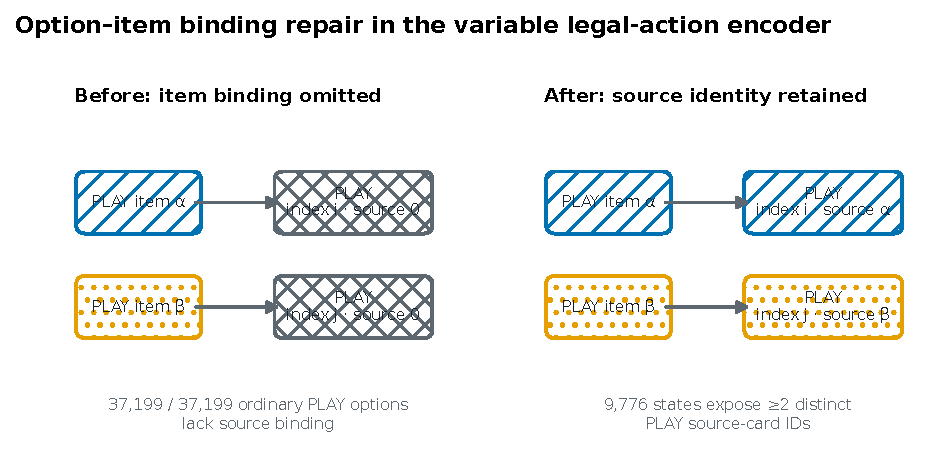
\includegraphics[width=0.92\textwidth]{figures/fig02_action_aliasing.pdf}
  \caption{Case-study option--item binding.  The blind encoder retains position
  and other option attributes but assigns source identity zero; the repaired
  encoder binds the public identity at that position.  The retained audit found
  no exact within-state full-input collision, so the schematic depicts a missing
  relation rather than literal equality of complete option vectors.}
  \label{fig:binding}
\end{figure*}

\section{Historical gameplay and offline diagnostics}

The historical one-execution \CFour--\COne{} contrast used seven opponents,
both actual orders, and 200 pairs per stratum.  Candidate and control games
shared the scheduled engine seed, opponent, order, and physical seat, but ran as
separate process-pool tasks.  Its +2.786-point estimate and conditional interval
are retained only as motivation for the admission gate.  Opponent/order cells,
family summaries, and the post hoc five-opponent effects are secondary archival
descriptions, not confirmatory results.

Two offline diagnostics use different estimands.  Direct model scoring on
held-out-team feature rows and a retained replay evaluator ask which policy
matches a recorded action conditional on policy disagreement.  They do not
measure terminal gameplay value.  Historical-agent state distributions also
differ from those induced by the evaluated policies; this is the general
distribution-shift concern motivating interactive imitation methods, although
this study does not implement DAgger or claim its guarantees
\cite{ross2011dagger}.  Episode rather than decision identifiers are the
resampling clusters.  These diagnostics are excluded from the abstract and do
not substitute for the \PEVL{} gates.

\section{Negative results, exclusions, and provenance}

Two bounded null experiments retain sufficient raw evidence for reaggregation.
An actual-second two-turn temporal takeover covered 1,200 paired units and had
a +0.083-point estimate with interval $[-2.000,+2.167]$.  A second-own-turn
sequence oracle covered 960 worlds in 60 root clusters and had a +0.313-point
estimate with interval $[-1.458,+1.979]$.  These results constrain their exact
procedures and fixed opponents, not temporal policies or planning generally.

Project summaries also mention actor-only PPO, expected-Q labeling, an older
Turn Director, historical meta-weighted aggregates, and missing evaluation
waves.  Exact rows, weights, or packages needed for independent reconstruction
do not survive, so their numerical claims are excluded rather than promoted
from prose.  An earlier collision audit grouped option signatures across
unrelated observations and was rejected; within-state grouping yields zero
exact full-input collisions.  These exclusions demonstrate the same evidence
discipline as \PEVL{} but are not framework validation experiments.

\bibliography{references}

\end{document}
